\documentclass[a4paper, amsfonts, amssymb, amsmath, reprint, showkeys, nofootinbib, twoside]{revtex4-1}
\usepackage[english]{babel}
\usepackage[utf8]{inputenc}
\usepackage[colorinlistoftodos, color=green!40, prependcaption]{todonotes}
\usepackage[pdftex, pdftitle={Article}, pdfauthor={Author}]{hyperref}
\usepackage{amsthm}
\usepackage{mathtools}
\usepackage{physics}
\usepackage{xcolor}
\usepackage{caption}
\usepackage{hyperref}
\usepackage{multirow}
\usepackage{amsmath}
\usepackage{amssymb}
\usepackage{graphicx}
\graphicspath{Images}
\usepackage[left=23mm,right=13mm,top=35mm,columnsep=15pt]{geometry} 
\usepackage{adjustbox}
\usepackage{placeins}
\usepackage[T1]{fontenc}
\usepackage{float}
%\usepackage{longtable}
\usepackage{csquotes}
\usepackage{refstyle}
\usepackage{lipsum}
\usepackage{booktabs}

\begin{document}

\title{Gamma Ray Spectroscopy using Single and Multi Channel Analyzer}
\author{Swaroop Ramakant Avarsekar}
\email{swaroop.avarsekar@niser.ac.in}
\affiliation{School of Physical Sciences, National Institute of Science Education and Research, HBNI, Jatni -752050, India}
\date{\today}

\begin{abstract}
Gamma ray spectroscopy used for gamma ray detection and energy measurement. In this experiment, we study dependence of energy resolution of high voltage and determine the best operating voltage for scintillation detector. We also study $Cs^{137}$ spectrum and calculate the resolution for a given detector, using single and multi channel analyzer. $Co^{60}$ spectrum and its resolution is in terms of energy is calculated using MCA. We also calibrate gamma ray spectrometer and find unknown energy of a radioactive isotope. Mass absorption coefficient in aluminium for 662 keV gamma rays to be 0.085 $cm^2/g$
\end{abstract}
	
\keywords{Photoelectric effect, Resolution, Mass absorption coefficient, FWHM}
\maketitle
\section{Theory}
Three gamma ray interaction mechanism have real significance in gamma ray spectroscopy: Photoelectric effect, Compton scattering and pair production. In Photoelectric Absorption: The incident gamma-ray photon interacts with an atom of the absorbing substance during this process, totally dissipating and transferring its energy to one of the atom’s orbital electrons. Compton Scattering: The 

Compton scattering process allows an incoming gamma-ray photon to interact with a single free electron in the absorber. An intense recoil electron is created as a result of the photon’s sudden direction change and transfer of some of its initial energy to the electron from which it dispersed.

Pair production: The process refers to the formation of an electron-positron pair at the point of total disappearance of the incident gamma-ray photon and takes place in the strong electric field close to the protons in the nuclei of the absorbing material.

A single-channel analyzer (SCA) is a device to measure the energy of charged particles. It works by using a magnetic field to bend the trajectory of the charged particle and a detector to measure the particle’s energy which can be calculated by knowing the radius of curvature of the particle’s trajectory and the magnetic field strength. Scintillation detector determines the energy level of an emission.

The resolution denotes degree of boardening which is given by,
\begin{equation}
	\text{Resolution}=\frac{Peak}{FWHM}100\%
\end{equation}

Both resolution and fwhm are important for NaI scintillation detectors. The one voltage at which resolution is low, is the operating voltage of the device. This is done by plotting applied voltage versus resolution and finding minima.

Multi channel Analyzer is a digital device to measure energy of charged particles which work on magnetic field to bend trajectory of the charged particle, followed by detectors to measure the particles energy. The particle's energy is quantised into no. of channels allowing for a more detailed energy spectrum is obtained. 

From Beer-Lambert's Law, decrease in intensity of radiation passes through absorber is given,
\begin{equation}
	I=I_oe^{-mx}
\end{equation}

$I$, $I_o$ is intensity of the before and after absorber, m is the total mass absorption coefficient, x is density thickness which is product of density and thickness. Half value layer is defined as density thickness of the absorbing material that will reduce the original intensity by half. 

\section{Experiment and Analysis}
Refer attached table for details.

\subsection{SCA}
FWHM was obtained from Gaussian fitting the data with different applied voltages and resolution was calculated from equation (1). The minima of plot for applied voltage and resolution is the operating voltage shown in figure 6. Plots for LLD versus counts are shown in figures 1,2,3,4 and 5. 

\begin{figure}[H]
	\centering
	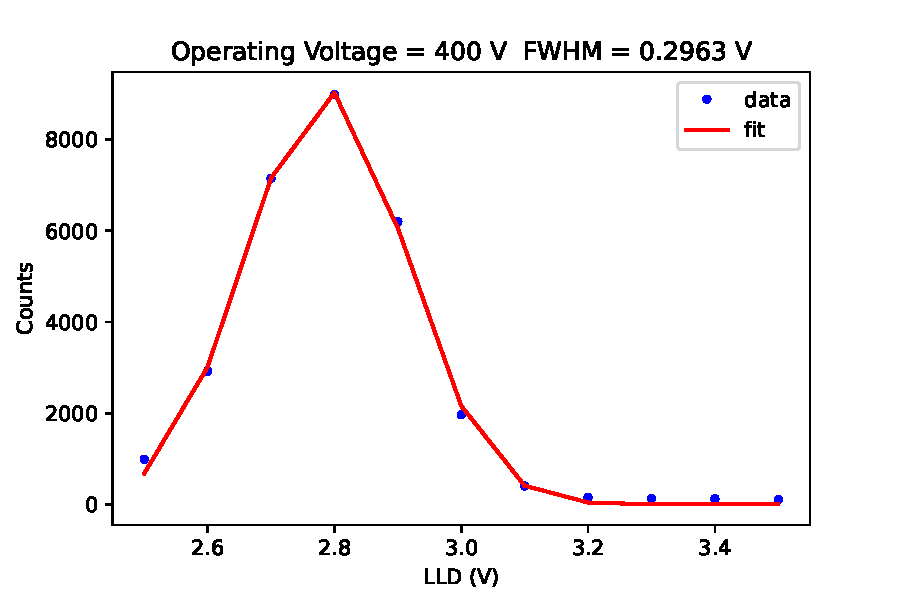
\includegraphics[scale=0.6]{1}
	\caption{LLD v/s Count for 400 V}
\end{figure}

\begin{figure}[H]
	\centering
	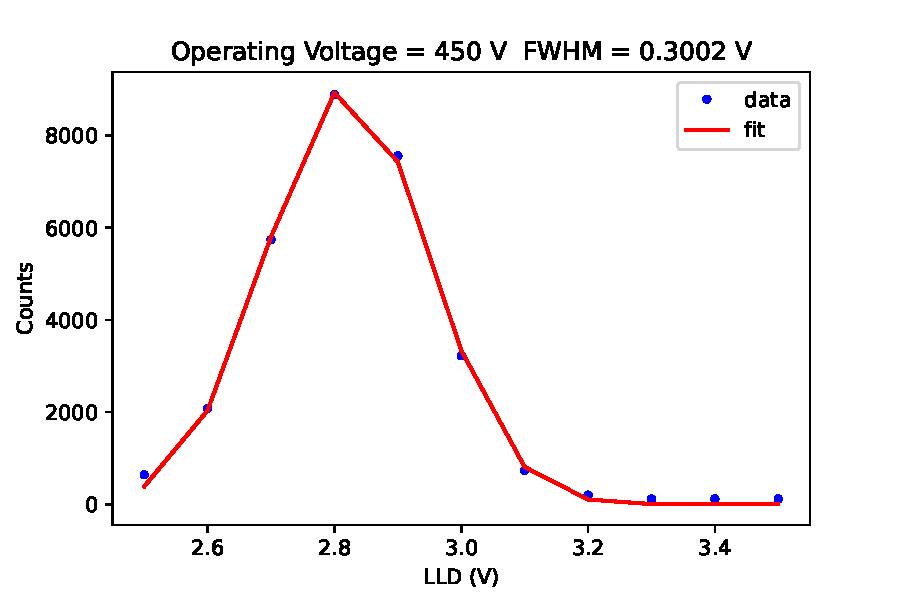
\includegraphics[scale=0.6]{2}
	\caption{LLD v/s Count for 450 V}
\end{figure}

\begin{figure}[H]
	\centering
	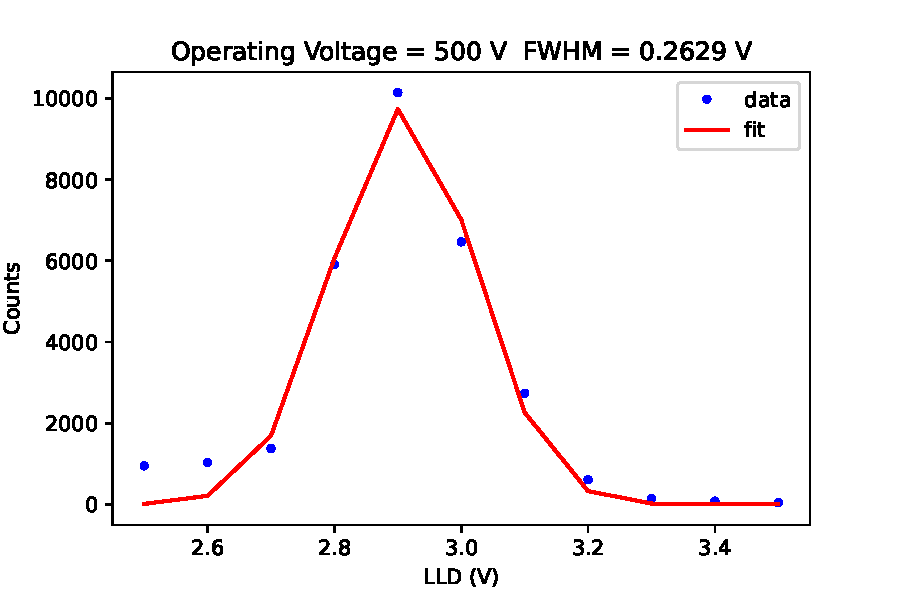
\includegraphics[scale=0.6]{3}
	\caption{LLD v/s Count for 500 V}
\end{figure}

\begin{figure}[H]
	\centering
	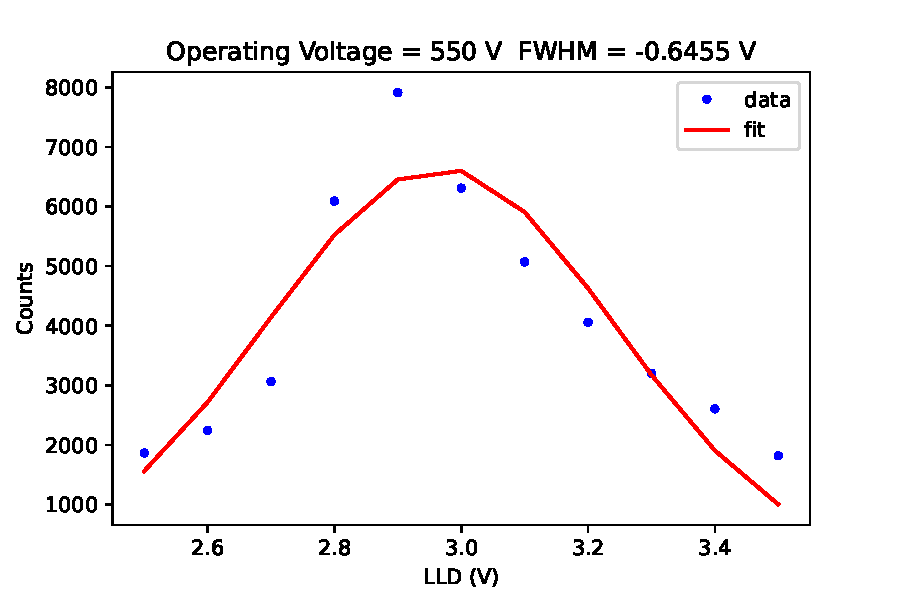
\includegraphics[scale=0.6]{4}
	\caption{LLD v/s Count for 550 V}
\end{figure}

\begin{figure}[H]
	\centering
	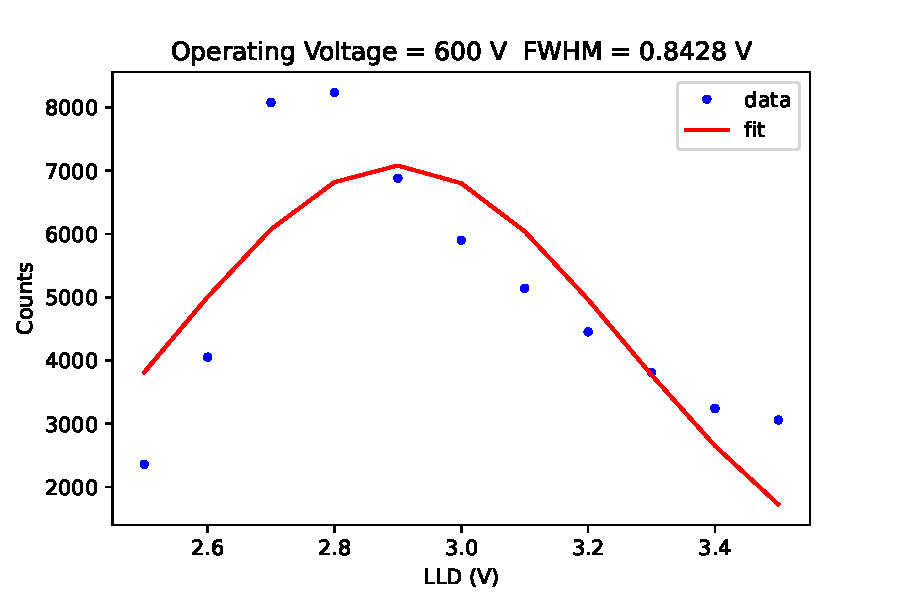
\includegraphics[scale=0.6]{5}
	\caption{LLD v/s Count for 600 V}
\end{figure}

\begin{figure}[H]
	\centering
	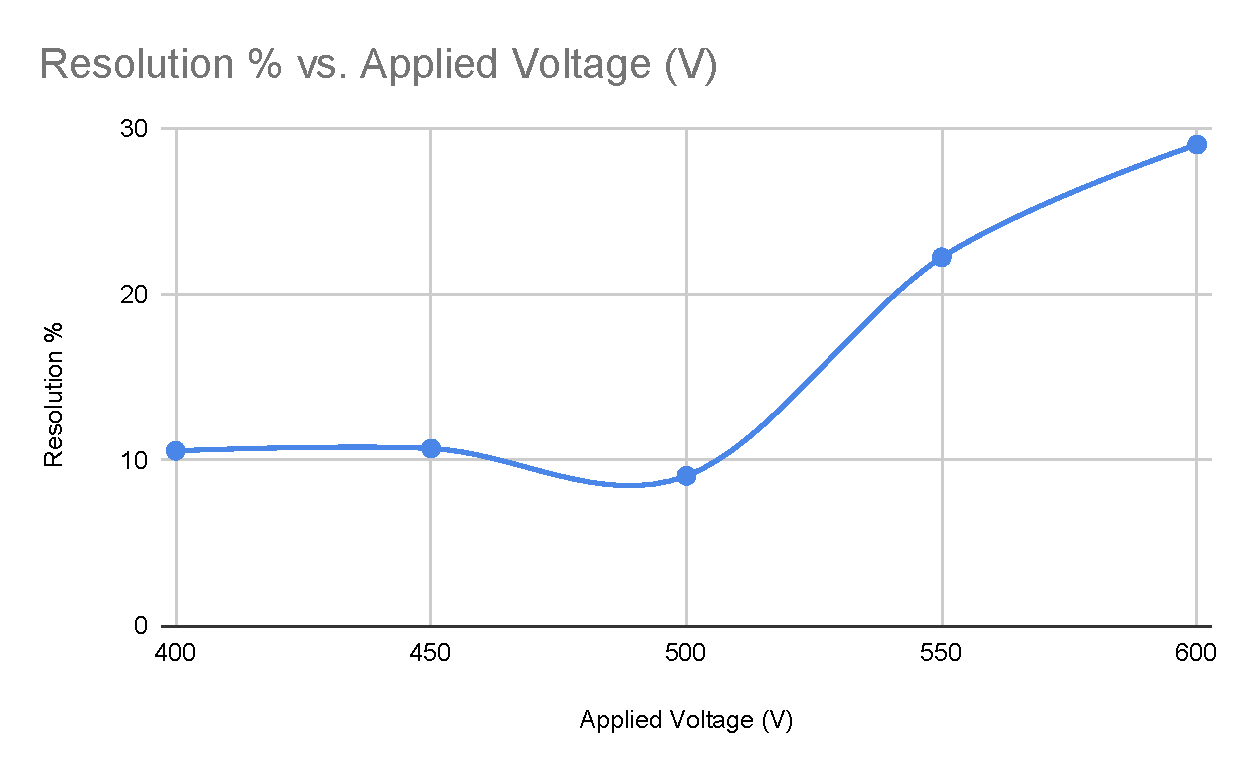
\includegraphics[scale=0.45]{6}
	\caption{Applied voltage versus Resolution}
\end{figure}

\begin{table}[H]
	\centering
	\caption{FWHM v/s resolution to determine operating voltage}
	\label{t1}
		\begin{tabular}{|c|c|c|}
			\hline
			Applied Voltage (V) & FWHM (V) & Resolution \% \\ \hline
			400                 & 0.2963   & 10.58214286   \\ \hline
			450                 & 0.3002   & 10.72142857   \\ \hline
			500                 & 0.2629   & 9.065517241   \\ \hline
			550                 & 0.6455   & 22.25862069   \\ \hline
			600                 & 0.8428   & 29.06206897   \\ \hline
		\end{tabular}
\end{table}

In figure (6), It is seen that resolution is lower in 500 V. Therefore we mark 500 V as our operating voltage.

\begin{figure}[H]
	\centering
	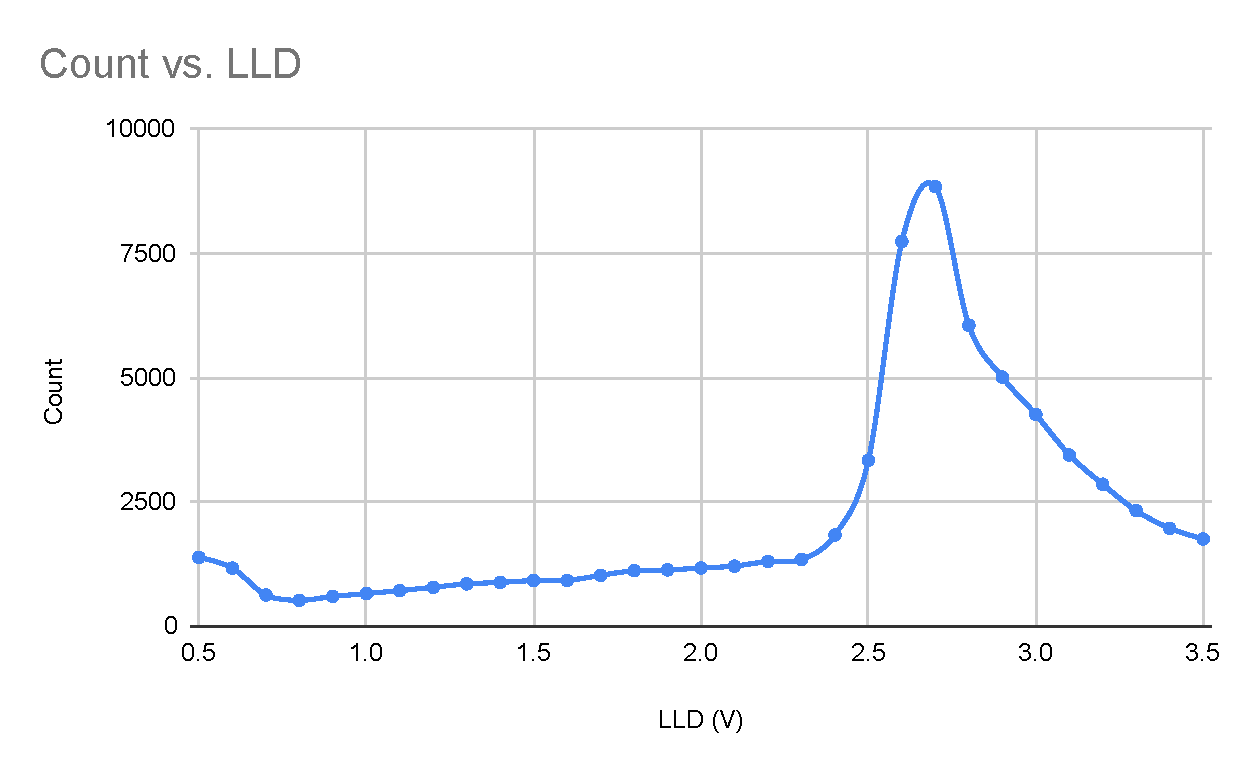
\includegraphics[scale=0.45]{7}
	\caption{Cs-137 Spectrum from SCA}
\end{figure}

In Cs-137 plot, the Resolution is 13.44 \%,
where fwhm is $\approx0.39$ V as shown in figure 7.

\subsection{MCA}

We obtained operating voltage from previous section. Here calibration is done using Cs-137, and calculate the resolution,

\begin{figure}[H]
	\centering
	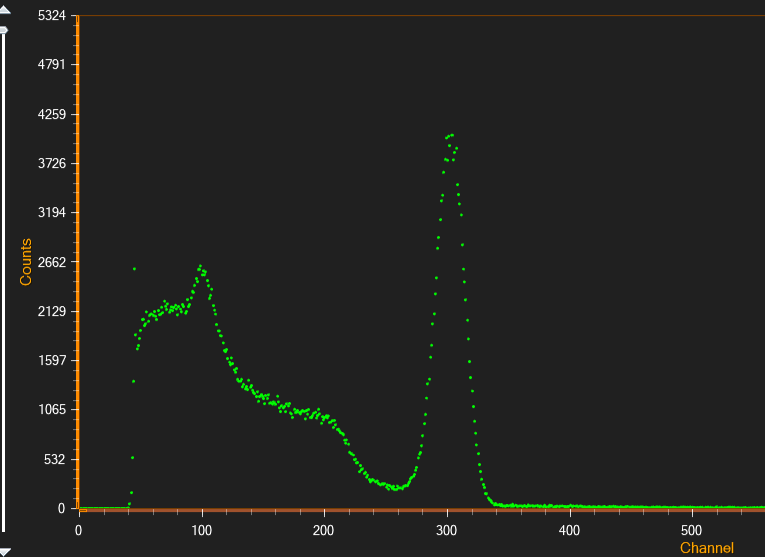
\includegraphics[width=\columnwidth]{Cs Spec}
	\caption{Cs-137 Spectrum from MCA}
\end{figure}

\begin{figure}[H]
	\centering
	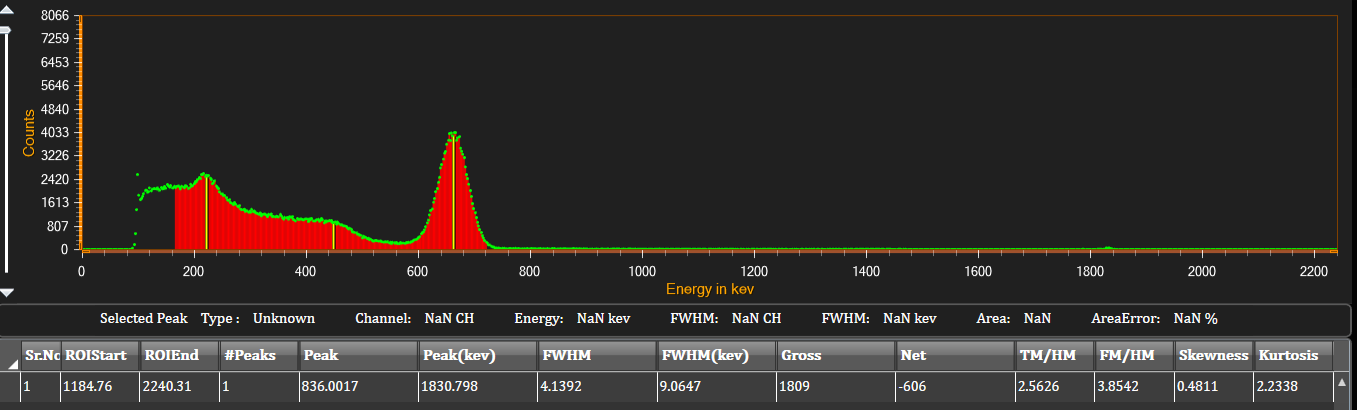
\includegraphics[scale=0.2]{cal}
	\caption{Calibrated Cs-137 Spectrum from MCA}
\end{figure}

\begin{table}[H]
	\centering
	\caption{Cs-137 spectrum ROI data}
	\label{t2}
	\begin{tabular}{|c|c|}
		\hline
		Energy (keV) & 662          \\ \hline
		Channel      & 302.2906799  \\ \hline
		FW(CH)       & 27.05643082  \\ \hline
		FW(EN)       & 59.2521019   \\ \hline
		Area         & 109106.1172  \\ \hline
		Area Error   & 0.4376287758 \\ \hline
	\end{tabular}
\end{table}

Resolution can be calculated from the above data as,
\begin{equation}
	\text{Resolution}=\frac{FW(CH)}{\text{Peak Channel}} 100\%=8.95\%
\end{equation}

Now we calculate the resolution of scintillation detector with Co-60. Refer figure 9 and 10 for spectrum and report.

\begin{figure*}[h]
	\centering
	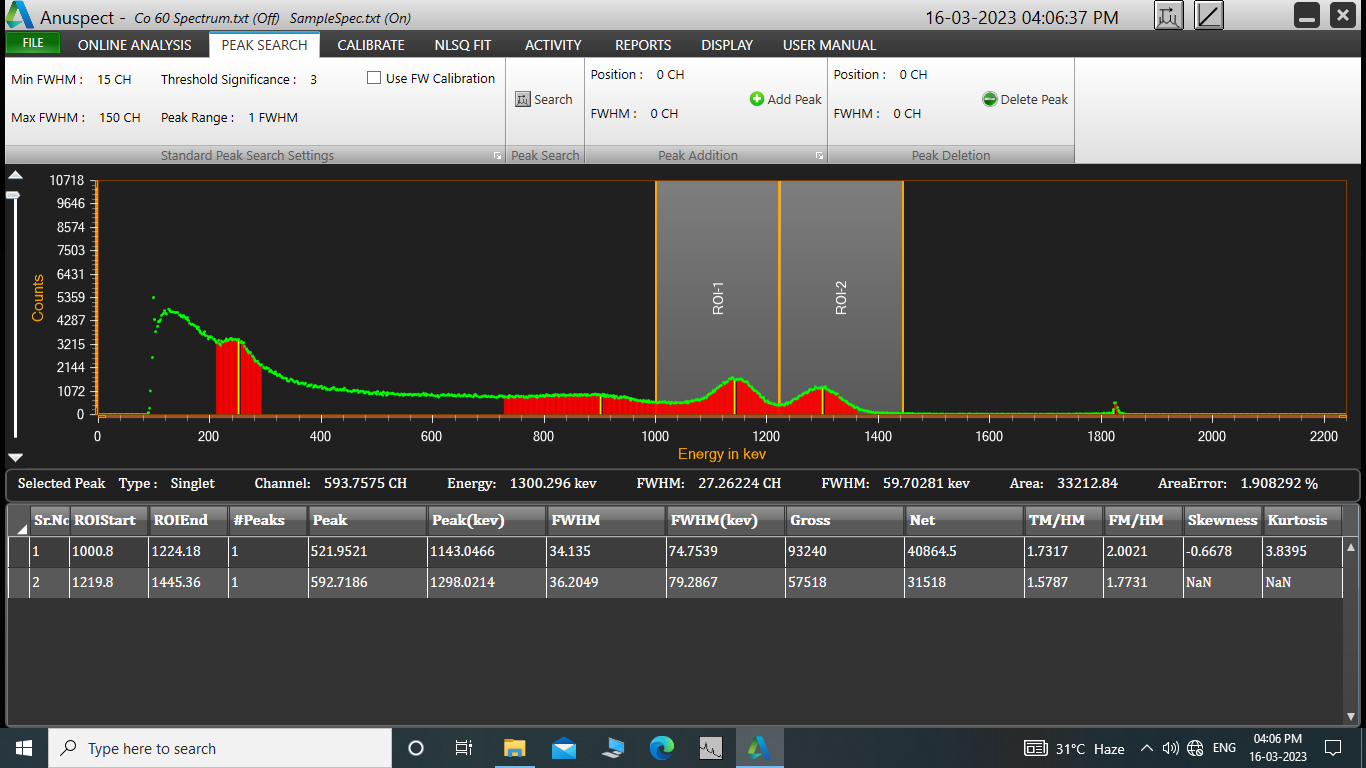
\includegraphics[width=\textwidth]{Co 60}
	\caption{Co-60 Spectrum from MCA}
\end{figure*}

\begin{figure*}[h]
	\centering
	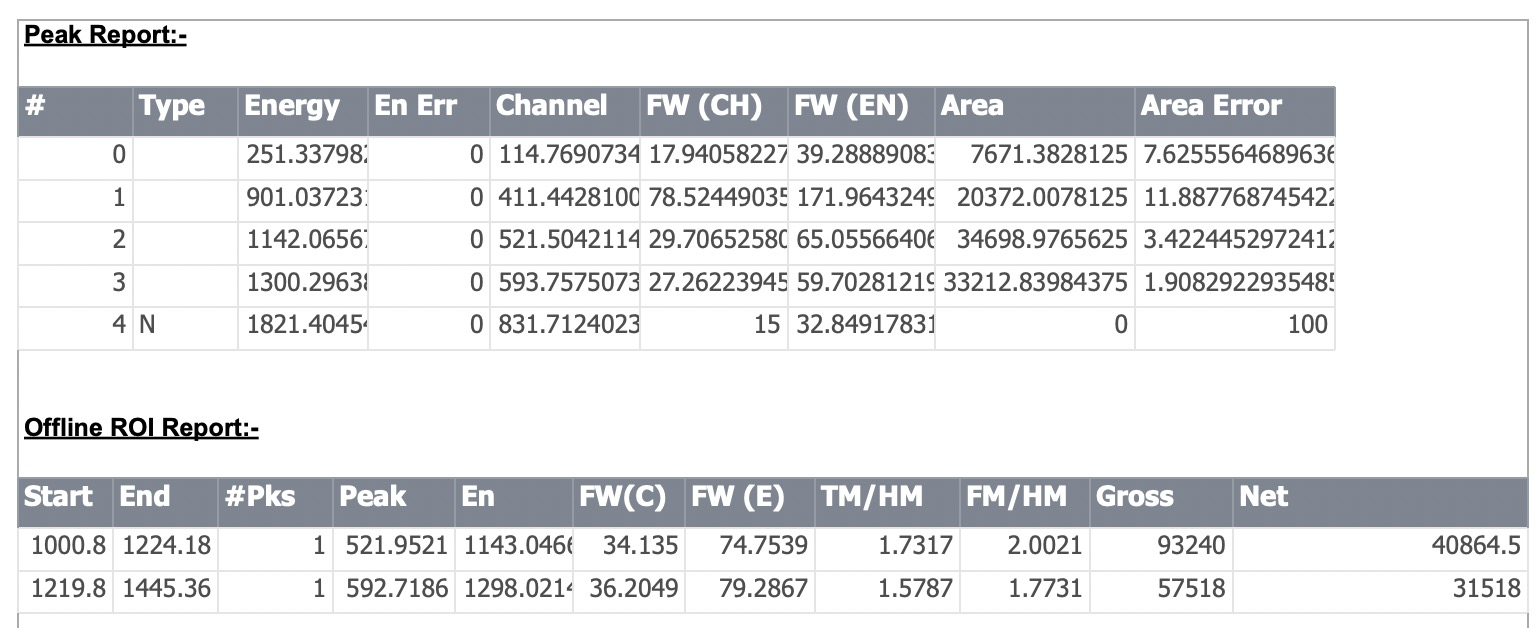
\includegraphics[width=\textwidth]{co}
	\caption{Co-60 Spectrum from report}
\end{figure*}

For 1.142 MeV and 1.3 MeV the peak channels are 521.5 and 593.75. 

The energy difference is 
\begin{align}
	\text{Energy difference}=1.300-1.142=0.158= 158 keV\\
	\text{Channel difference}=593.75-521.5=72.25~ \text{channel }\\
	\text{One Channel corresponds to}=158/72.25=2.18~ keV
\end{align}

From ROI-1, we get FW(CH) as 29.70 and ROI-2, FW(CH) is 27.62. 

FWHM in terms of energy
\begin{align}
FWHM_1=29.7*2.18=64.74 keV\\
FWHM_2=27.62*2.18=60.21 keV
\end{align}

\begin{align}
	\text{Resolution}&=\frac{FWHM}{\text{Peak Ch Energy}}=\frac{64.74}{662}.100\%=9.78\%\\
	\text{Resolution}&=\frac{60.21}{662}.100\%=9.09\%
\end{align}

Now, to study the energy calibration of gamma ray spectrometer with different energy sources. Three sources Ba-133, Cs-137 and Co-60 are used. The spectrum can be seen in  Figure 11. With calibrating the energies from peak channels, It is seen that the peak channels of the gamma rays is proportional to energy of the gamma ray as shown in Figure (11). 

\begin{figure*}[h]
	\centering
	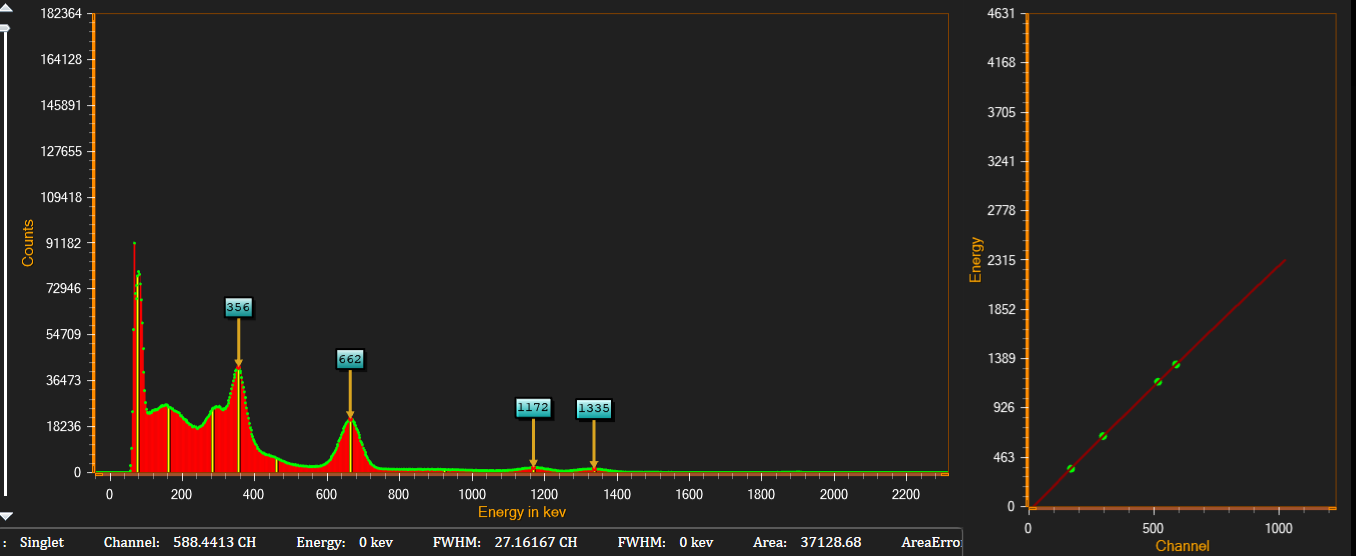
\includegraphics[width=\textwidth, height=\columnwidth,angle=90]{th}
	\caption{Ba-133, Cs-137 and Co-60 Spectrum from MCA along with the plot of linear relationship of Energy and peak channel number}
\end{figure*}

To determine the unknown energy of radioactive isotope, we take the previous calibration from the previously used sources and use Na-22 (unknown source). The spectrum is shown in Figure (12).

\begin{figure*}[h]
	\centering
	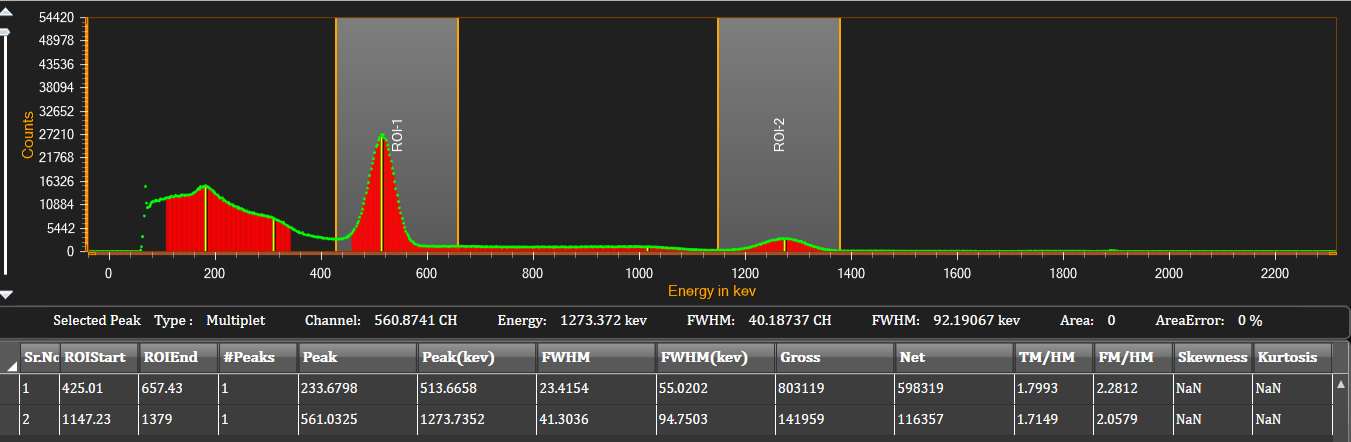
\includegraphics[width=\textheight,height=\columnwidth,angle=90]{Na}
	\caption{Na-22 Spectrum from MCA }
\end{figure*}

\begin{figure}[H]
	\centering
	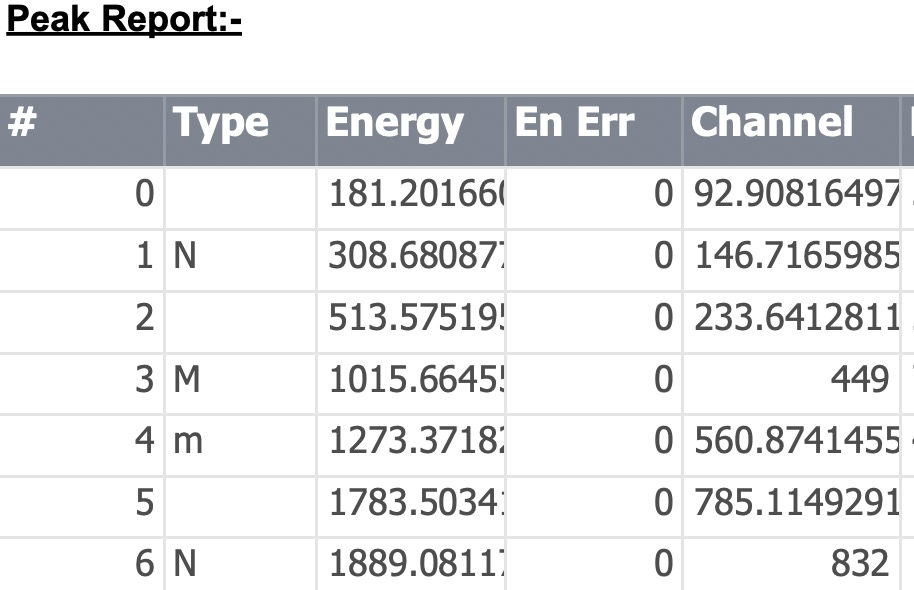
\includegraphics[width=\columnwidth]{ca}
	\caption{Na-22 Spectrum report from MCA}
\end{figure}

We expect a 511 keV photon when radionuclide emits positrons as part of decay and 1275 keV. The excited neon state of Na-22 passes into ground state with 1275 keV gamma ray emitted. 

From the spectrum we see peak at 513.66 keV and 1273.73 keV which is close to expected and can be claimed that the used source is Na-22.

The relative error RE is calculated as 
\begin{align}
	RE_1=\frac{513.66-511}{511}.100\%=0.52\%\\
	RE_2=\frac{1275-1273.73}{1275}.100\%=0.01\%
\end{align}


We use gamma spectrometer to measure the mass absorption coefficient of aluminium plates for 662 keV gamma rays. The calculate the Half value layer or thickness HVL, is the thickness when net count reduces by half. The background spectrum was also taken to reduce the systematic error. The backgrund count was 219.

\begin{table}[H]
	\centering
	\caption{Calculation of mass absorption coefficient of Al}
	\label{t3}
	\begin{tabular}{|c|c|}
		\hline
		Thickness (cm) & Net counts \\ \hline
		0              & 45315      \\ \hline
		0.6            & 39030      \\ \hline
		1.2            & 33930      \\ \hline
		1.8            & 30507      \\ \hline
		2.4            & 27536      \\ \hline
		3              & 23125      \\ \hline
		3.6            & 20450      \\ \hline
		4.2            & 18465      \\ \hline
		4.8            & 15452      \\ \hline
		5.4            & 14016      \\ \hline
		6              & 12891      \\ \hline
		6.6            & 11235      \\ \hline
	\end{tabular}
\end{table}

\begin{figure}[H]
	\centering
	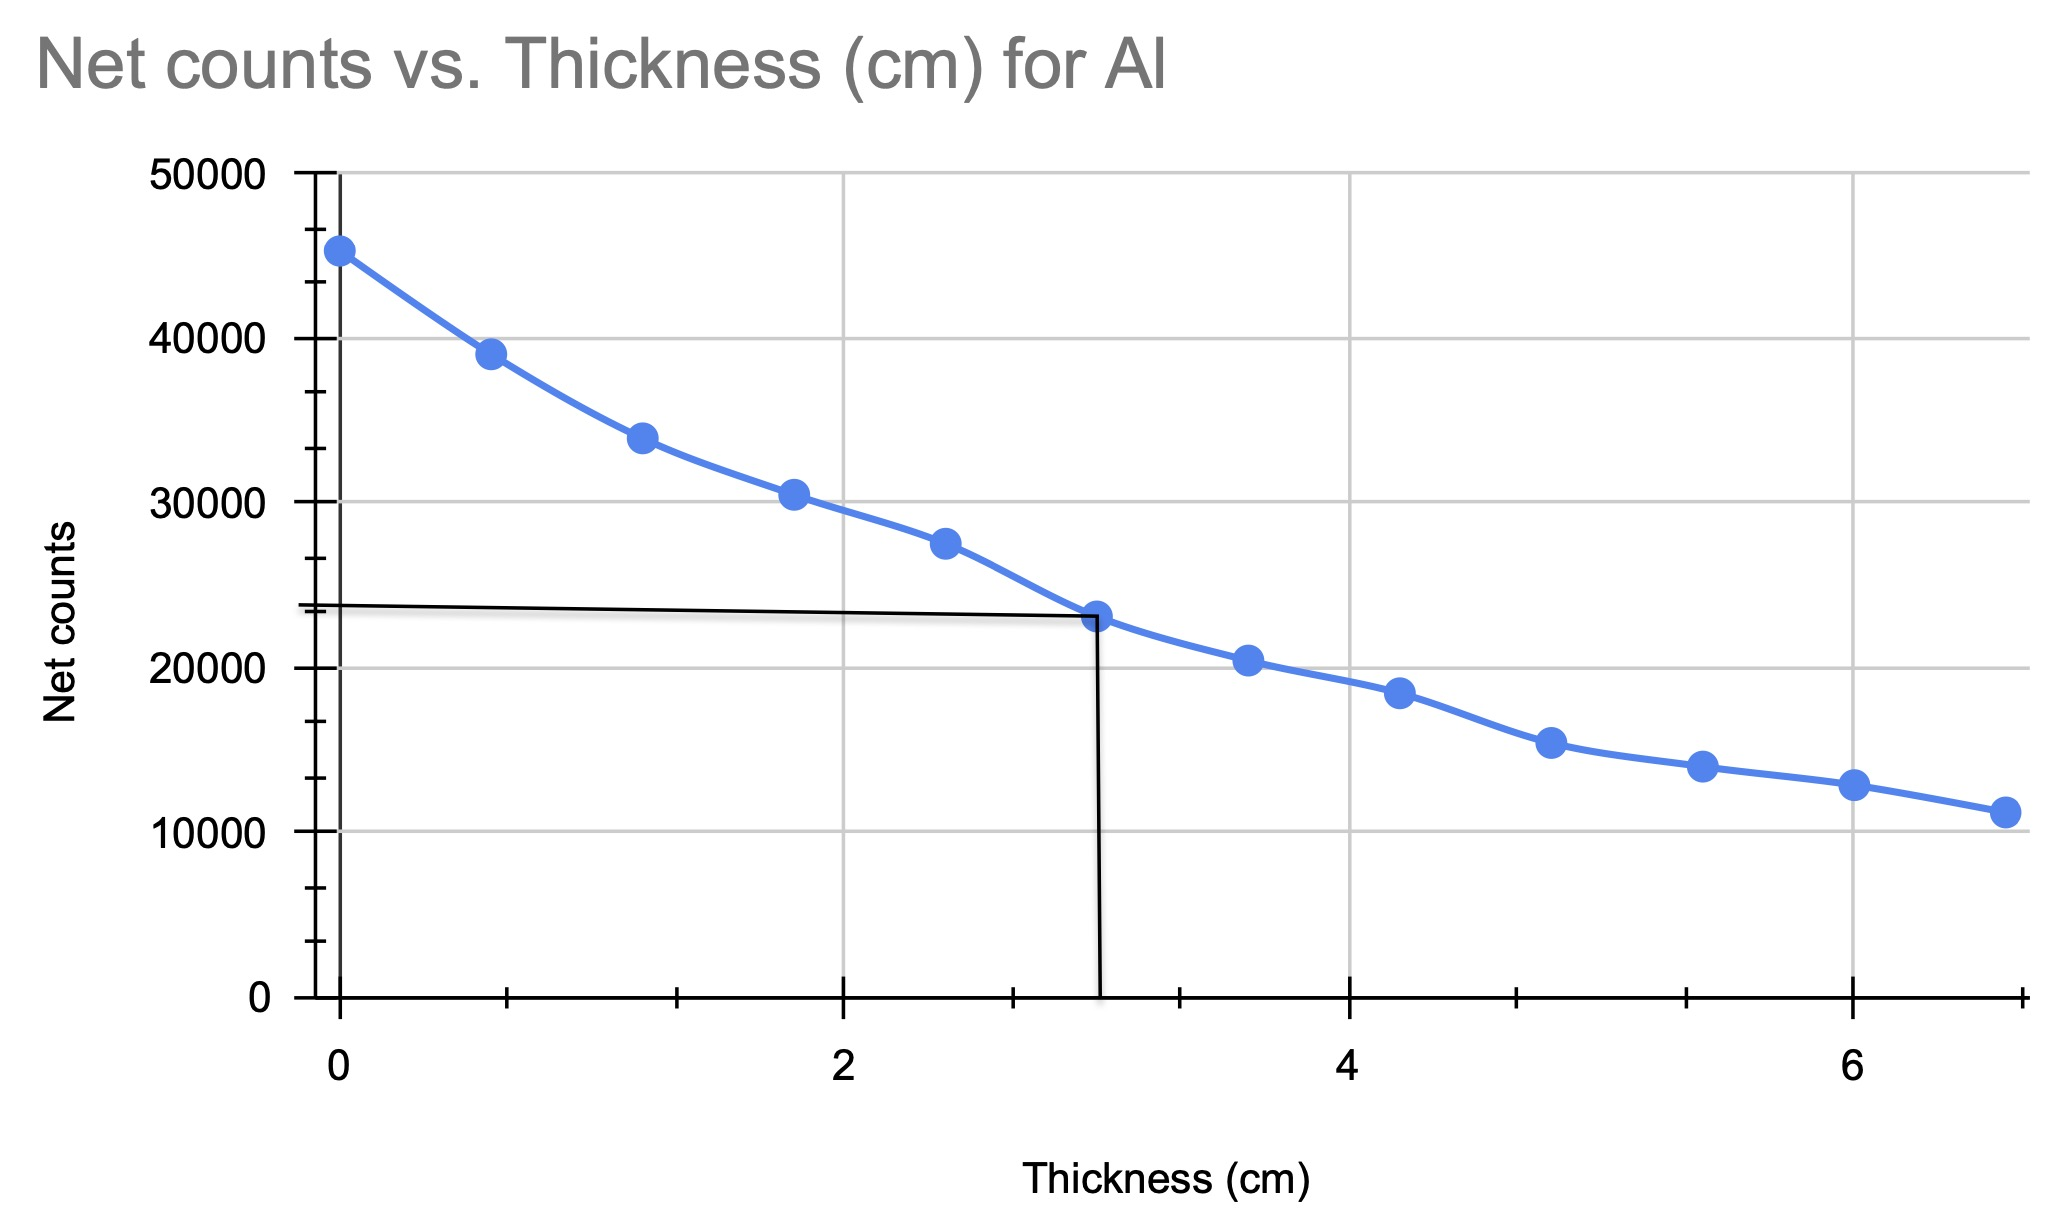
\includegraphics[width=\columnwidth]{mc}
	\caption{Count v/s Thickness graph for Al}
\end{figure}

From Figure 14, it is seen that HVL is 3 cm.

The density of aluminium is $2.7 g/cm^3$. Therefore, density thickness,
\begin{equation}
	\text{Density Thickness}=3\times2.7=8.1 g/cm^2
\end{equation}

Therefore, the mass absorption coefficient is, 
\begin{equation}
	m=\frac{0.693}{8.1}=0.085 cm^2/g
\end{equation}

\begin{widetext}
	\begin{minipage}{\linewidth}
		\begin{figure}[H]
			\centering
			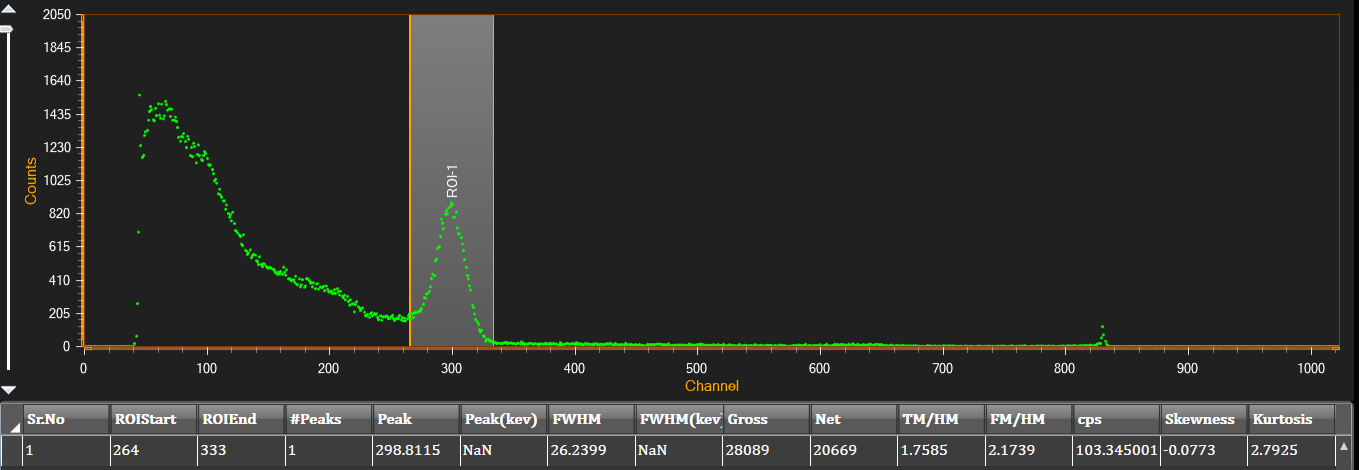
\includegraphics[width=\linewidth]{ma}
			\label{fig:sample}
			\caption{A spectrum from the absoption due to Al}
		\end{figure}    
	\end{minipage}
\end{widetext}

\section{Conclusion}
This experiment, we study dependence of energy resolution of high voltage and determine the best operating voltage for scintillation detector using SCA. The best operating voltage was found to be 500 V since the resolution is minimum at that point compared to other voltages. The resolution was calculated from FWHM from the Gaussian fit of the peak. We also study $Cs^{137}$ spectrum and calculate the resolution for a given detector, using single and multi channel analyzer. $Co^{60}$ spectrum and its resolution is in terms of energy is calculated using MCA. We also calibrate gamma ray spectrometer and find unknown energy of a radioactive isotope. The unknown radioactive source closely resembled to Na-22 with the energy peaks at 513.66$\pm$0.52\% keV and 1273$\pm$0.01 keV. Mass absorption coefficient in aluminium for 662 keV gamma rays to be 0.085 $cm^2/g$. It is seen that the counts with increasing thickness decreases gradually.

Several errors have contributed in this experiment especially in SCA method. The tuning, shaping and adjusting gain are the things which one should take care of. The variations in pulse amplitude and shape due to temperature fluctuations and noise. Statistical fluctuations in counts for low count rates. The experiment can be improved by taking larger time for the detector to read the counts. On should also properly align and adjust he aluminium slabs to cover the detector to avoid unwanted direct counts to creep in.

\section{References}
\begin{enumerate}
\item{\url{NISER lab manual}}
\item{\url{https://ns.ph.liv.ac.uk/~ajb/radiometrics/glossary/sodium22.html}}
\item {\url{https://www.ld-didactic.de/software/524221en/Content/Appendix/Na22.htm}}
\item {\url{https://en.wikipedia.org/wiki/Aluminium}}
\end{enumerate}

\end{document}